\section{Pixie}

\subsection{توضیحات کلی}

در این بخش، با استفاده از الگوریتم‌های خانواده‌ی 
\lr{Page Rank}
و در واقع با الگوریتمی شبیه به الگوریتم 
Pixie 
داده‌ ها را تحلیل می‌کنیم. برای این کار، پس از تمیز‌کردن داده‌های اولیه، تنها 
ماشین‌های پرتردد را نگه می‌داریم. 

برای استفاده از الگوریتم، یک گراف دو بخشی در نظر می‌گیریم، که یک سمت‌ آن 
ماشین‌ها قرار دارند و سمت دیگر آن دوربین‌ها. سپس بین هر ماشین، و هر دوربینی 
که آن ماشین از آن رد شده، یک یال در نظر می‌گیریم که وزن آن برابر با تعداد 
بار‌هایی است که دوربین آن ماشین را دیده است. سپس تمام یال‌ها را به صورت یک لیست مجاورت نگه می‌داریم (که به کمک 
آن می‌توانیم یال‌های خروجی از هر راس را به دست آوریم). 

حال الگوریتم 
Pixie
را پیاده‌سازی می‌کنیم. این الگوریتم هم می‌تواند از یک دوربین شروع شود، و هم از یک ماشین. بدون کاستن از کلیت تنها یک سمت آن را توضیح می‌دهیم، اما کد هر دو سمت در فایل
jupyter
موجود است.

با شروع از دوربین اولیه، لیست تمامی ماشین‌های دیده‌شده 
در آن دوربین را انتخاب می‌کنیم و به صورت تصادفی به یکی از ماشین‌ها می‌رویم. سپس 
باز‌هم لیست تمام دوربین‌هایی که آن ماشین در آن‌ها دیده شده را در نظر می‌گیریم و 
تصادفی به یکی از آن دوربین‌ها می‌رویم. برای هر دوربین یک 
counter
نگه می‌داریم و هربار که از یک دوربین (روی گراف) عبور می‌کنیم، آن را یک واحد 
افزایش می‌دهیم. پس از طی شدن تعداد مرحله‌ای مشخص، لیست 
counter
ها را خروجی می‌دهیم. 

چند نکته‌ی حائز اهمیت در این الگوریتم وجود دارد. اول آن که 
لیست راس‌های سمت مقابل، واقعا به صورت «لیست» نگه داشته شده است. یعنی 
ممکن است عضوی تکراری داشته باشد. این کار از عمد صورت گرفته است، 
تا در واقع شانس انتخاب راس‌هایی با یال با وزن بیشتری وصل شده‌اند بیشتر شود. 
در واقع انتخاب راس سمت مقابل با این که تصادفی است، اما از یک توزیع احتمال پیروی 
می‌کند که احتمال انتخاب یال‌های با وزن بالا را متناسب با وزن آن 
افزایش می‌دهد. نکته‌ی بعدی نیز این است که به احتمال ثابتی، هر بار به راس 
اولیه برمی‌گردیم که این احتمال در کد من برابر با 
$0.2$
بوده است. 


\subsection{تحلیل نتایج}

حال که راجب نحوه‌ی پیاده‌سازی و کلیات این ایده صحبت کردیم، می‌توانیم بیشتر در مورد کاربرد‌های آن صحبت 
کنیم. 

اولین کاربردی که این الگوریتم دارد این است که می‌تواند دوربین‌هایی که از نظر 
فیزیکی به هم نزدیکند را پیدا کند. زیرا اگر دو دوربین به هم نزدیک باشند، در صورتی که 
یک ماشین در یکی از آن‌ها دیده شود، به احتمال بیشتری در دیگری نیز دیده می‌شود. 
دقت کنید که عواملی مثل نوع دوربین در اینجا تاثیر گذارند. یعنی شباهت دوربین‌ها در 
حالت کلی تنها وابسته به فاصله‌ی فیزیکی نیست. در ادامه به این مورد بیشتر خواهم پرداخت. 

در حالت کلی، اگر یک دوربین به عنوان ورودی داده شود، می‌توانیم شبیه‌ترین دوربین‌ها به آن را 
با این روش به دست آوریم. برای مثال یک نمونه از خروجی الگوریتم به صورت زیر است: 

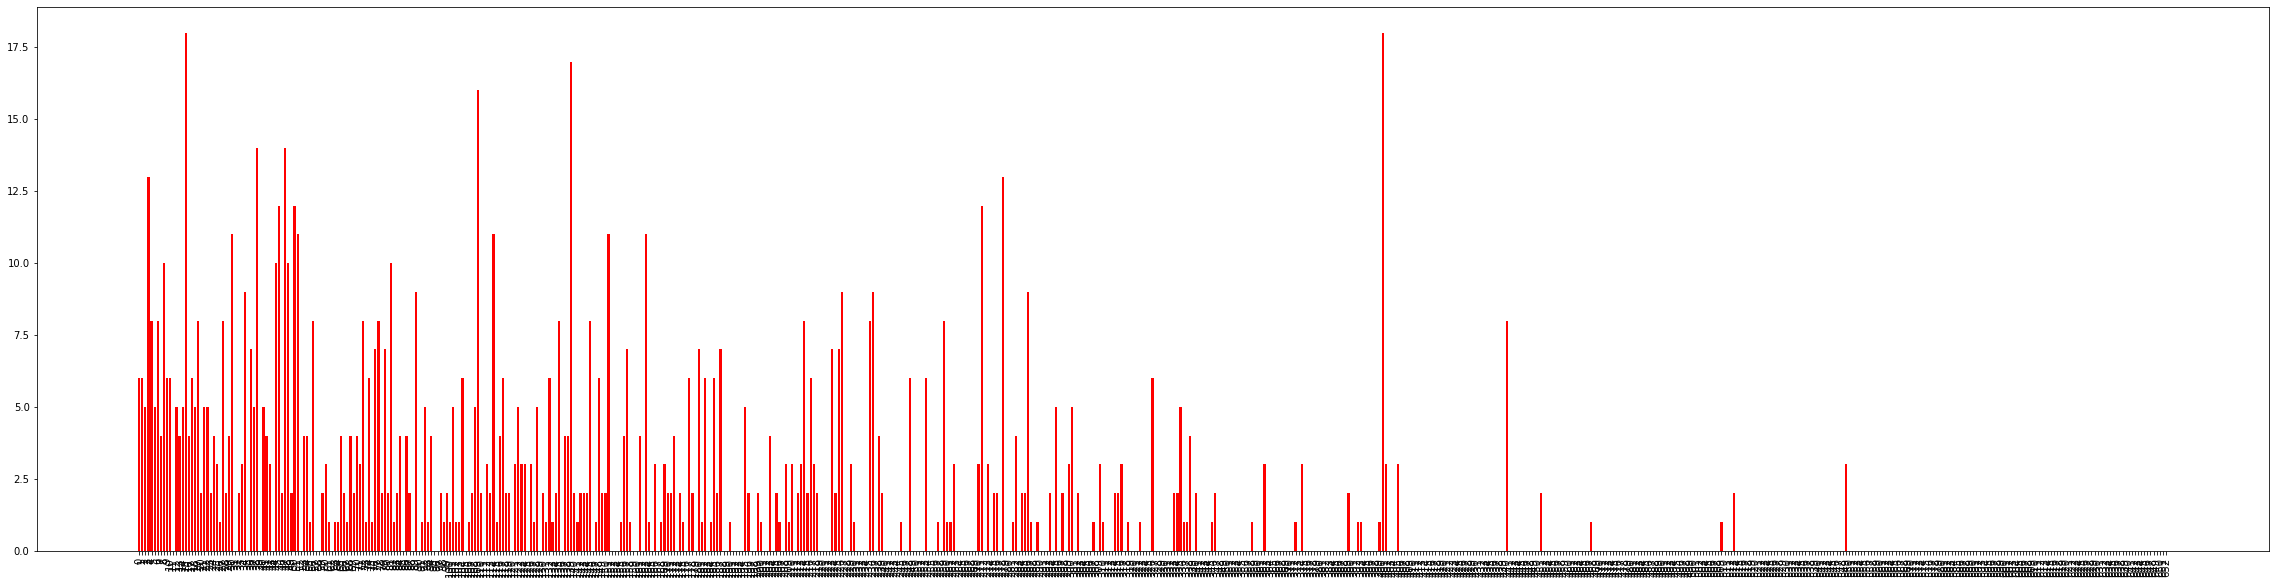
\includegraphics[scale=0.2]{images/Pixie/1.png}


همانطور که می‌بینید، به کمک این اطلاعات می‌توانیم دوربین‌های نزدیک را بیابیم. 
حال اگر یک گراف رسم کنیم، که هر راس آن یک دوربین باشد، و هر دوربین را به 
چند دوربین نزدیک خود وصل کنیم، می‌توانیم نقشه‌ای حدودی‌ از شهر داشته باشیم (حتی اگر موقعیت جغرافیایی دوربین‌ها را نداشته باشیم). 
«چند»
دوربین نزدیک نیز می‌تواند عددی بین ۲ تا ۶ باشد (برای نتایج منطقی تر). دقت کنید که 
با این روش، اگر تنها لیست مکان دوربین‌ها را داشته باشیم، و اسم دوربین‌ها کد 
گذاری شده باشد، احتمال دارد بتوانیم موقعیت دقیق هرکدام از دوربین‌ها را 
روی نقشه بیابیم! پس این روش در حالت کلی می‌تواند به ما دوربین‌های مجاور را 
بدهد اما کار‌های دیگری نیز مانند آنچه گفته شد می‌توان انجام داد.

نکته‌ی مهمی که حائز اهمیت است، این است که «نزدیکی» دوربین‌ها با تحلیل من 
لزوما نمی‌تواند به معنای نزدیکی فیزیکی باشد. زیرا اگر دو دوربین هردو تخلفات یکسانی را ثبت کنند، 
احتمال بیشتری وجود دارد که ماشین‌های یکسان را ثبت کنند. یعنی «نزدیکی» در 
این تحلیل می‌تواند نزدیک بودن نوع دوربین‌ها باشد. یک مثال از این اتفاق را 
می‌توانید در کد من ببینید. در بخشی از کد، نزدیک‌ترین دوربین‌ها به دوربین کوئری خود را در نظر گرفتم 
و نوع آن‌ها را چاپ کردم. نوع دوربین کوئری من ۸۱ بود، یعنی دوربین محدوده‌ی طرح 
ترافیک. و همانطوری که در نتایج دیده می‌شود، ۱۰ دوربین نزدیک همگی از نوع ۸۱ یا ۲۸۳ هستند 
که نوع ۲۸۳ نیز به معنی دوربین طرح زوج و فرد است (که در واقع یک دوربین محدوده طرح ترافیک است). 

با استاده از مطلب بالا، می‌توانید ببینید که ما بدون دانستن اطلاعتی مانند نوع دوربین، می‌توانیم 
دوربین‌های با نوع مشابه و نزدیک به هم را پیدا کنیم. یعنی اگر نوع دوربین‌ها به ما داده نشده بود 
احتمالا می‌توانستیم دوربین‌ها را بر اساس شباهت‌هایی که از این الگوریتم به دست می‌آید دسته بندی کنیم. 

نکته‌ی دیگری که تحلیل بالا مشخص می‌کند این است که اگر دوربین‌های نوع‌های مختلف را حذف کنیم و فقط 
آن‌هایی را نگه داریم که به صورت کلی ثبت می‌کنند (نه به دلیل اتفاق خاصی، مانند نوع ماشین یا یک تخلف خاص) 
آنگاه می‌توانیم ایده‌ای که در بالا مطرح شد را بهتر پیاده سازی کنیم، و دیگر دوربین‌های 
نزدیک واقعا به معنی دوربین‌هایی هستند که از نظر فیزیکی به هم نزدیکند و به 
این صورت می‌توانیم نقشه‌ی گراف شهر را بکشیم. 

حال به الگوریتم از سمت دیگر نگاه کنید. این الگوریتم می‌تواند ماشین‌های «نزدیک» 
به هم را تشخیص دهد. دقیقا مانند بالا، نزدیک بودن ماشین‌ها می‌تواند معیار‌های معیار‌های متفاوتی 
داشته باشد. برای مثال، اگر یک ماشین خاص را شناسایی کنیم که تعداد زیادی 
تخلف سرعت غیرمجاز دارد، با کمک این الگوریتم می‌توانیم ماشین‌هایی را بیابیم 
که الگوی حرکتی مشابهی با این ماشین دارند و در واقع ماشین‌هایی را بیابیم 
که رانندگی پرخطر دارند. تمام تحلیل‌های بالا را می‌توان برای این حالت نیز 
به کار گرفت و می‌توانیم ماشین‌هایی هم «نوع» را به دست بیاوریم. 

